\section{Testes e Resultados}

Após a implementação da ALU, foram realizados testes para cada uma das 16 operações especificadas. As simulações foram feitas utilizando o editor de formas de onda (VWF) do Quartus II, com diferentes valores de entrada para os sinais \texttt{a\_in}, \texttt{b\_in}, \texttt{c\_in} e \texttt{op\_sel}. Cada teste resultou em uma imagem capturada da simulação, localizada na pasta \texttt{Testes/} do projeto.

A seguir, são apresentados os resultados obtidos em cada operação, com a respectiva análise.

\subsection{Operações Aritméticas}

\begin{figure}[H]
\centering
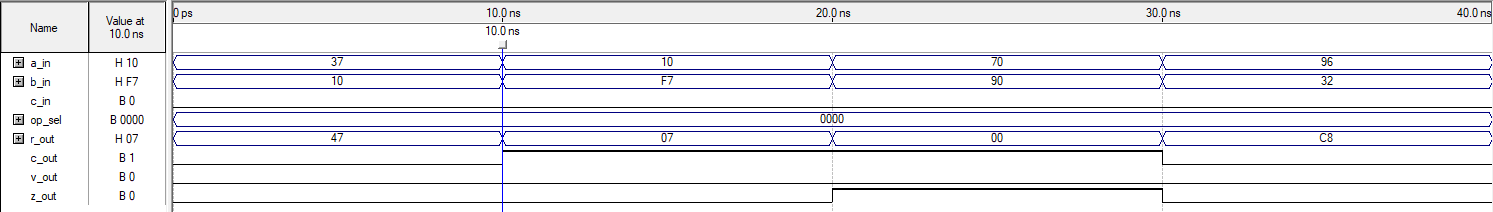
\includegraphics[width=\textwidth]{images/alu_0000.png}
\caption{Operação ADD (\texttt{op\_sel = 0000}): Soma sem carry-in}
\end{figure}

Nesta simulação, observa-se que o valor de \texttt{r\_out} corresponde corretamente à soma de \texttt{a\_in} e \texttt{b\_in}. O sinal \texttt{c\_out} indica a ocorrência (ou não) de carry, e \texttt{v\_out} sinaliza overflow quando aplicável.

\begin{figure}[H]
\centering
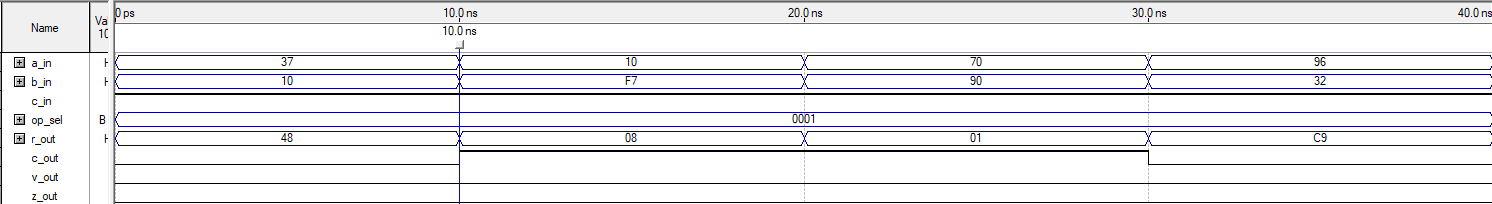
\includegraphics[width=\textwidth]{images/alu_0001_com_carry_in.png}
\caption{Operação ADDC (\texttt{op\_sel = 0001}): Soma com carry-in}
\end{figure}

\begin{figure}[H]
\centering
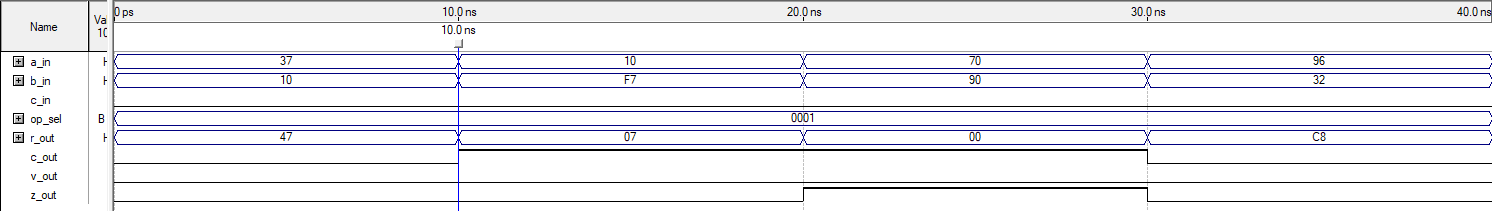
\includegraphics[width=\textwidth]{images/alu_0001_sem_carry_in.png}
\caption{Operação ADDC (\texttt{op\_sel = 0001}): Soma sem carry-in}
\end{figure}

Neste caso, o bit de carry-in (\texttt{c\_in}) é adicionado ao resultado, afetando tanto o valor de saída quanto o \texttt{c\_out} final.

\begin{figure}[H]
\centering
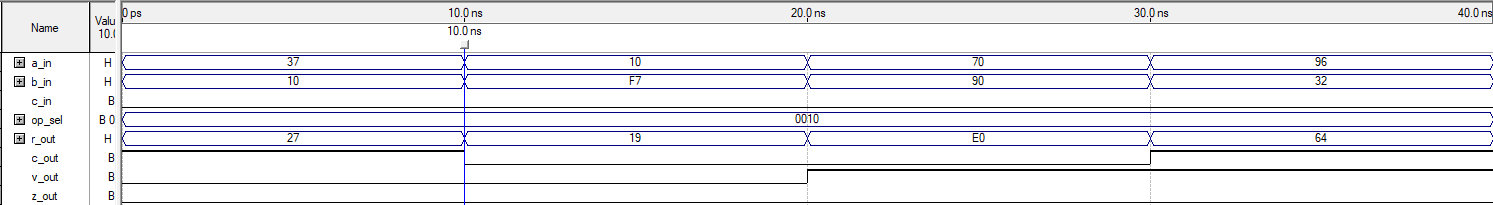
\includegraphics[width=\textwidth]{images/alu_0010.png}
\caption{Operação SUB (\texttt{op\_sel = 0010}): Subtração sem carry-in}
\end{figure}

A subtração simples de \texttt{a\_in} menos \texttt{b\_in} é realizada, e o \texttt{c\_out} representa o borrow.

\begin{figure}[H]
\centering
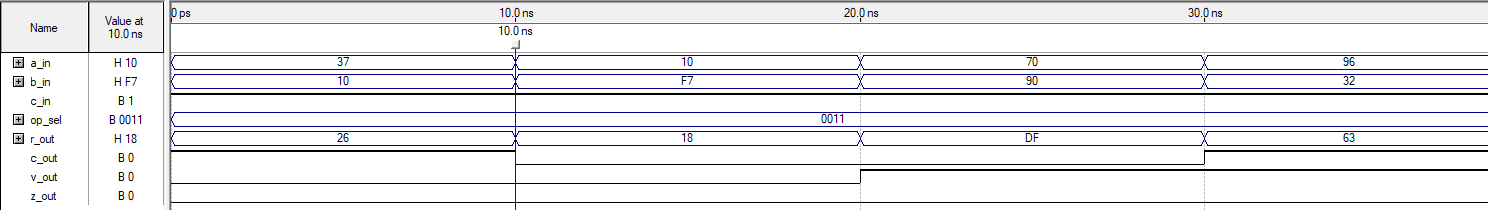
\includegraphics[width=\textwidth]{images/alu_0011_com_carry_in.png}
\caption{Operação SUBC (\texttt{op\_sel = 0011}): Subtração com carry-in}
\end{figure}

\begin{figure}[H]
\centering
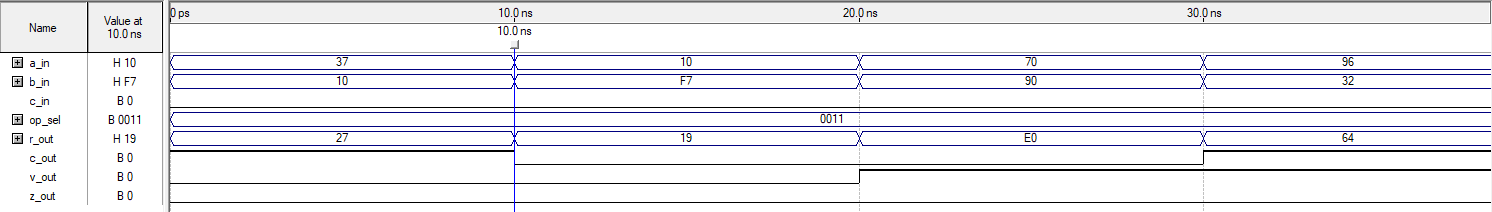
\includegraphics[width=\textwidth]{images/alu_0011_sem_carry_in.png}
\caption{Operação SUBC (\texttt{op\_sel = 0011}): Subtração sem carry-in}
\end{figure}

A subtração considera o carry-in como um decrementador adicional, afetando o resultado final e os sinais auxiliares.

\subsection{Operações Lógicas}

\begin{figure}[H]
\centering
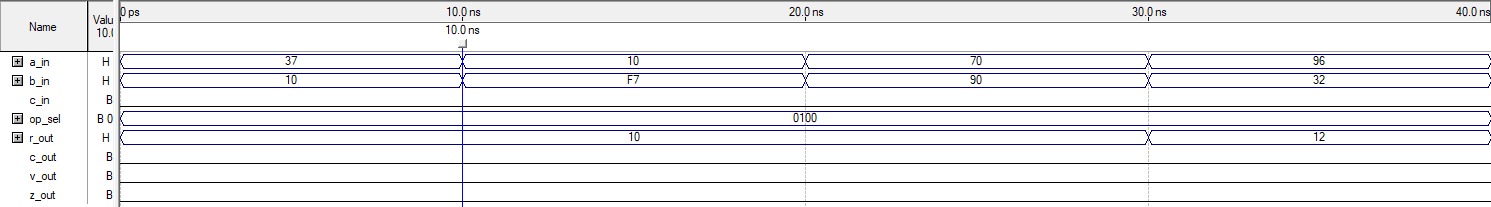
\includegraphics[width=\textwidth]{images/alu_0100.png}
\caption{Operação AND (\texttt{op\_sel = 0100})}
\end{figure}

A saída corresponde ao resultado do AND bit a bit entre os operandos \texttt{a\_in} e \texttt{b\_in}. O sinal \texttt{z\_out} indica se o resultado foi nulo.

\begin{figure}[H]
\centering
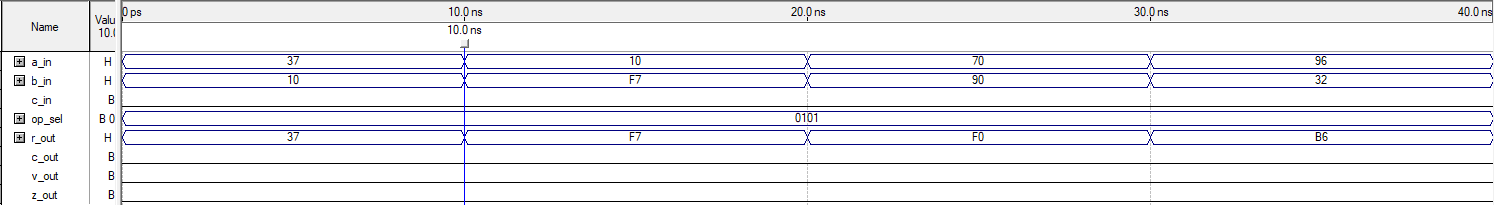
\includegraphics[width=\textwidth]{images/alu_0101.png}
\caption{Operação OR (\texttt{op\_sel = 0101})}
\end{figure}

Operação OR bit a bit entre os dois operandos, útil para ativar bits em paralelo.

\begin{figure}[H]
\centering
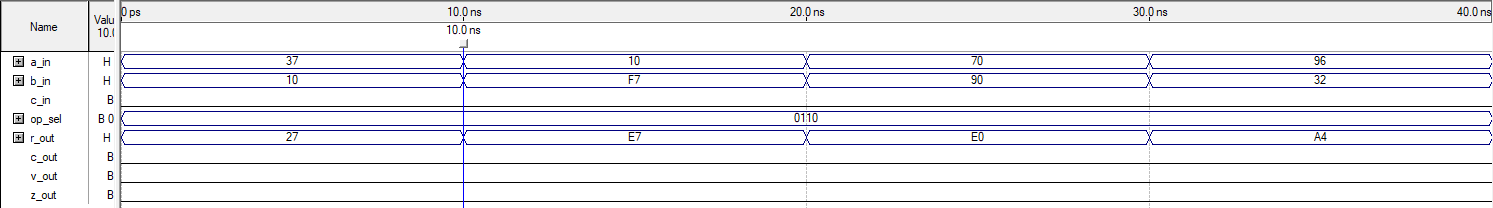
\includegraphics[width=\textwidth]{images/alu_0110.png}
\caption{Operação XOR (\texttt{op\_sel = 0110})}
\end{figure}

Realiza o XOR bit a bit, com o sinal de zero sendo ativado se todos os bits da saída forem '0'.

\begin{figure}[H]
\centering
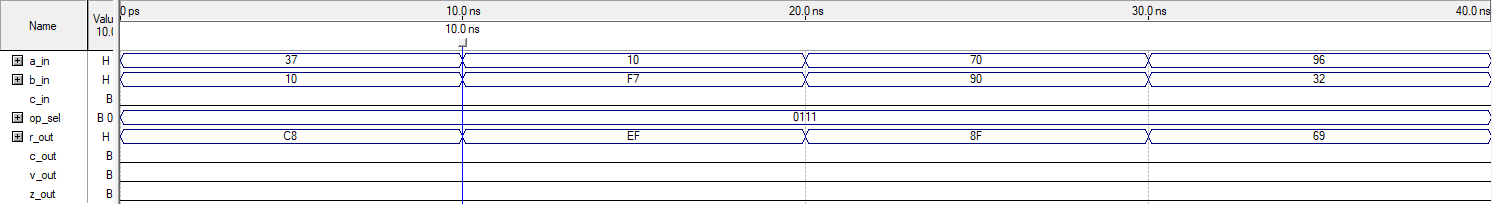
\includegraphics[width=\textwidth]{images/alu_0111.png}
\caption{Operação NOT (\texttt{op\_sel = 0111})}
\end{figure}

Complementa todos os bits de \texttt{a\_in}, ignorando \texttt{b\_in} e \texttt{c\_in}.

\subsection{Rotações e Deslocamentos}

\begin{figure}[H]
\centering
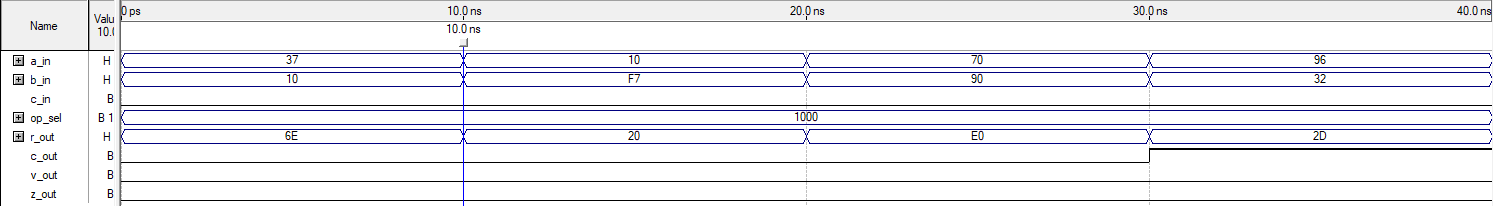
\includegraphics[width=\textwidth]{images/alu_1000.png}
\caption{Operação RL (\texttt{op\_sel = 1000}): Rotação para a esquerda}
\end{figure}

Rotaciona os bits de \texttt{a\_in} para a esquerda, com o bit mais significativo indo para a posição menos significativa.

\begin{figure}[H]
\centering
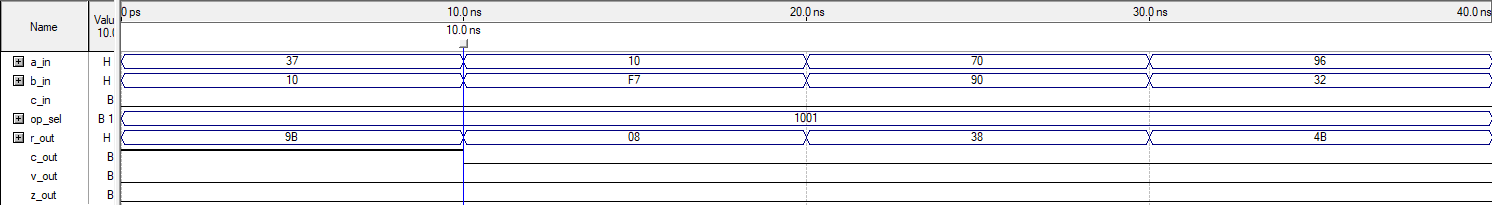
\includegraphics[width=\textwidth]{images/alu_1001.png}
\caption{Operação RR (\texttt{op\_sel = 1001}): Rotação para a direita}
\end{figure}

Rotação simples para a direita, levando o LSB para o MSB.

\begin{figure}[H]
\centering
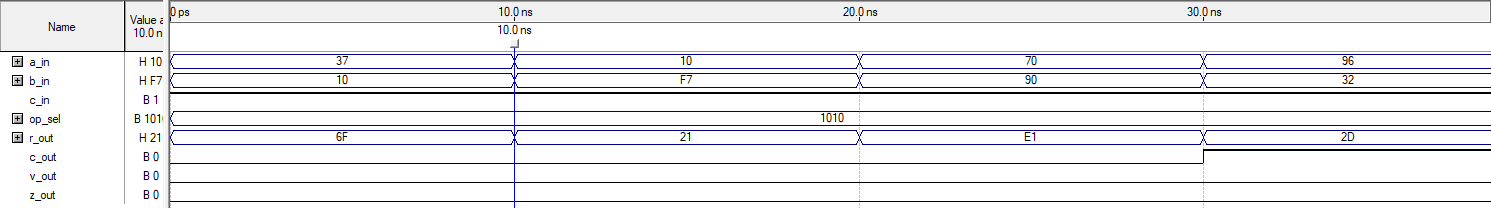
\includegraphics[width=\textwidth]{images/alu_1010_com_carry_in.png}
\caption{Operação RLC (\texttt{op\_sel = 1010}): Rotação à esquerda via carry}
\end{figure}

\begin{figure}[H]
\centering
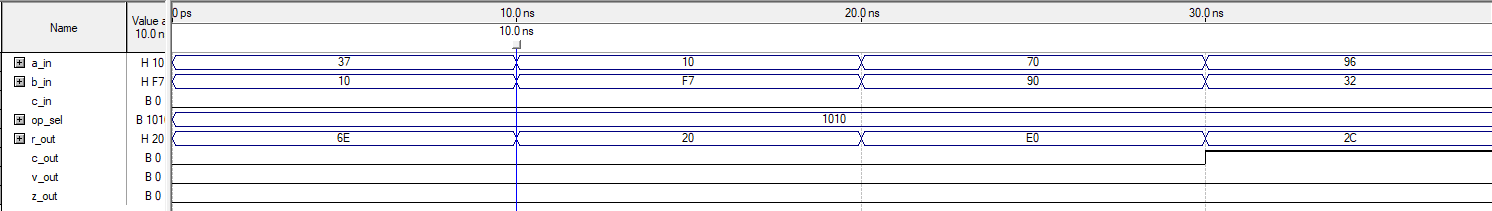
\includegraphics[width=\textwidth]{images/alu_1010_sem_carry_in.png}
\caption{Operação RLC (\texttt{op\_sel = 1010}): Rotação à esquerda sem carry}
\end{figure}

Aqui, o bit de carry-in é inserido como LSB, e o MSB de \texttt{a\_in} torna-se o \texttt{c\_out}.

\begin{figure}[H]
\centering
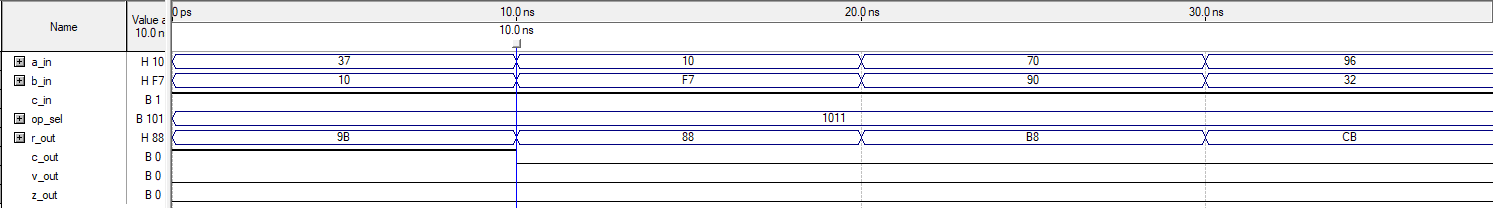
\includegraphics[width=\textwidth]{images/alu_1011_com_carry_in.png}
\caption{Operação RRC (\texttt{op\_sel = 1011}): Rotação à direita via carry}
\end{figure}

\begin{figure}[H]
\centering
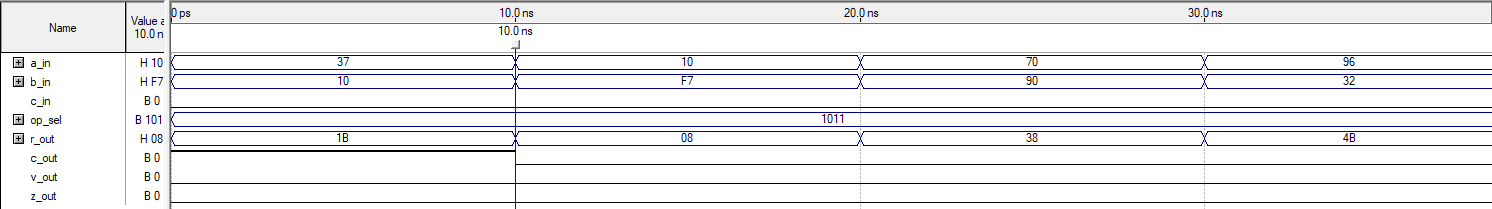
\includegraphics[width=\textwidth]{images/alu_1011_sem_carry_in.png}
\caption{Operação RRC (\texttt{op\_sel = 1011}): Rotação à direita sem carry}
\end{figure}

Similar à RLC, mas rotacionando para a direita. O carry-in ocupa o MSB, e o LSB vira \texttt{c\_out}.

\begin{figure}[H]
\centering
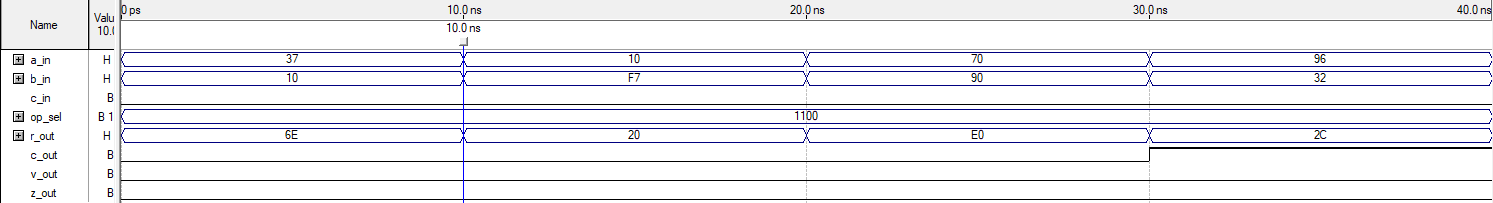
\includegraphics[width=\textwidth]{images/alu_1100.png}
\caption{Operação SLL (\texttt{op\_sel = 1100}): Deslocamento lógico à esquerda}
\end{figure}

Desloca os bits à esquerda e insere zero no LSB.

\begin{figure}[H]
\centering
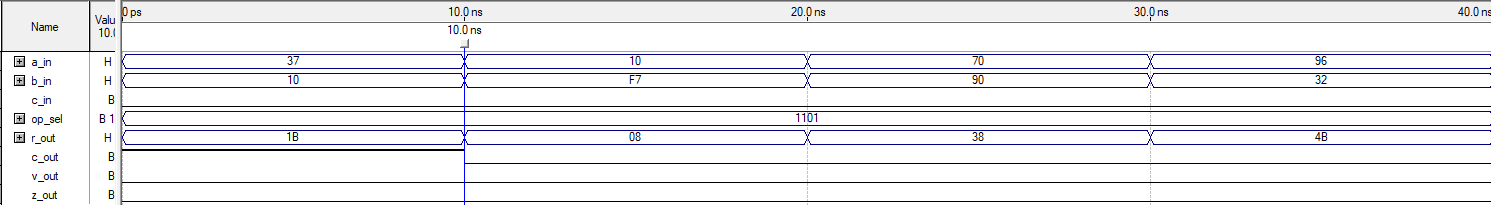
\includegraphics[width=\textwidth]{images/alu_1101.png}
\caption{Operação SRL (\texttt{op\_sel = 1101}): Deslocamento lógico à direita}
\end{figure}

Desloca os bits à direita, preenchendo o MSB com zero.

\begin{figure}[H]
\centering
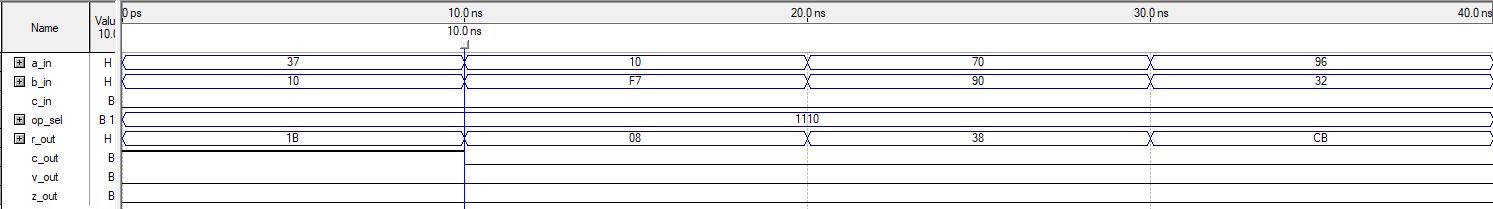
\includegraphics[width=\textwidth]{images/alu_1110.png}
\caption{Operação SRA (\texttt{op\_sel = 1110}): Deslocamento aritmético à direita}
\end{figure}

Mantém o bit de sinal (MSB) ao deslocar bits à direita.

\subsection{Bypass}

\begin{figure}[H]
\centering
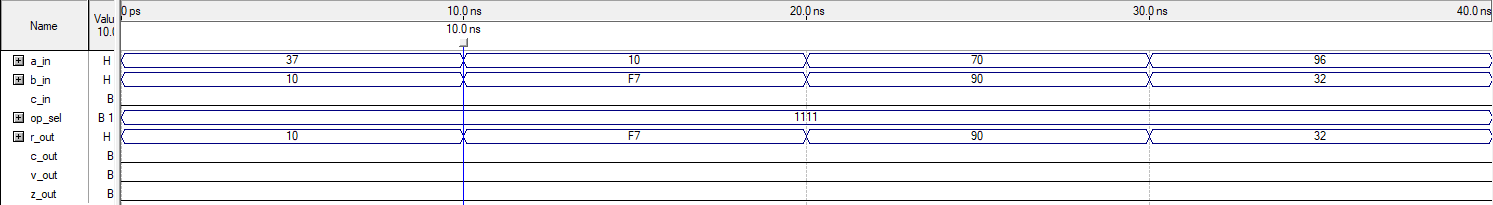
\includegraphics[width=\textwidth]{images/alu_1111.png}
\caption{Operação PASS\_B (\texttt{op\_sel = 1111}): Passagem direta de \texttt{b\_in}}
\end{figure}

Nesta operação, o valor de \texttt{b\_in} é passado diretamente para a saída \texttt{r\_out}, ignorando \texttt{a\_in} e \texttt{c\_in}.